\hypertarget{apr__thread__pool_8h}{}\section{/usr/local/src/github/\+Codebase/httpd-\/2.4.29/srclib/apr-\/util/include/apr\+\_\+thread\+\_\+pool.h File Reference}
\label{apr__thread__pool_8h}\index{/usr/local/src/github/\+Codebase/httpd-\/2.\+4.\+29/srclib/apr-\/util/include/apr\+\_\+thread\+\_\+pool.\+h@{/usr/local/src/github/\+Codebase/httpd-\/2.\+4.\+29/srclib/apr-\/util/include/apr\+\_\+thread\+\_\+pool.\+h}}


A\+PR Thread Pool Library.  


{\ttfamily \#include \char`\"{}apu.\+h\char`\"{}}\\*
{\ttfamily \#include \char`\"{}apr\+\_\+thread\+\_\+proc.\+h\char`\"{}}\\*
Include dependency graph for apr\+\_\+thread\+\_\+pool.\+h\+:
\nopagebreak
\begin{figure}[H]
\begin{center}
\leavevmode
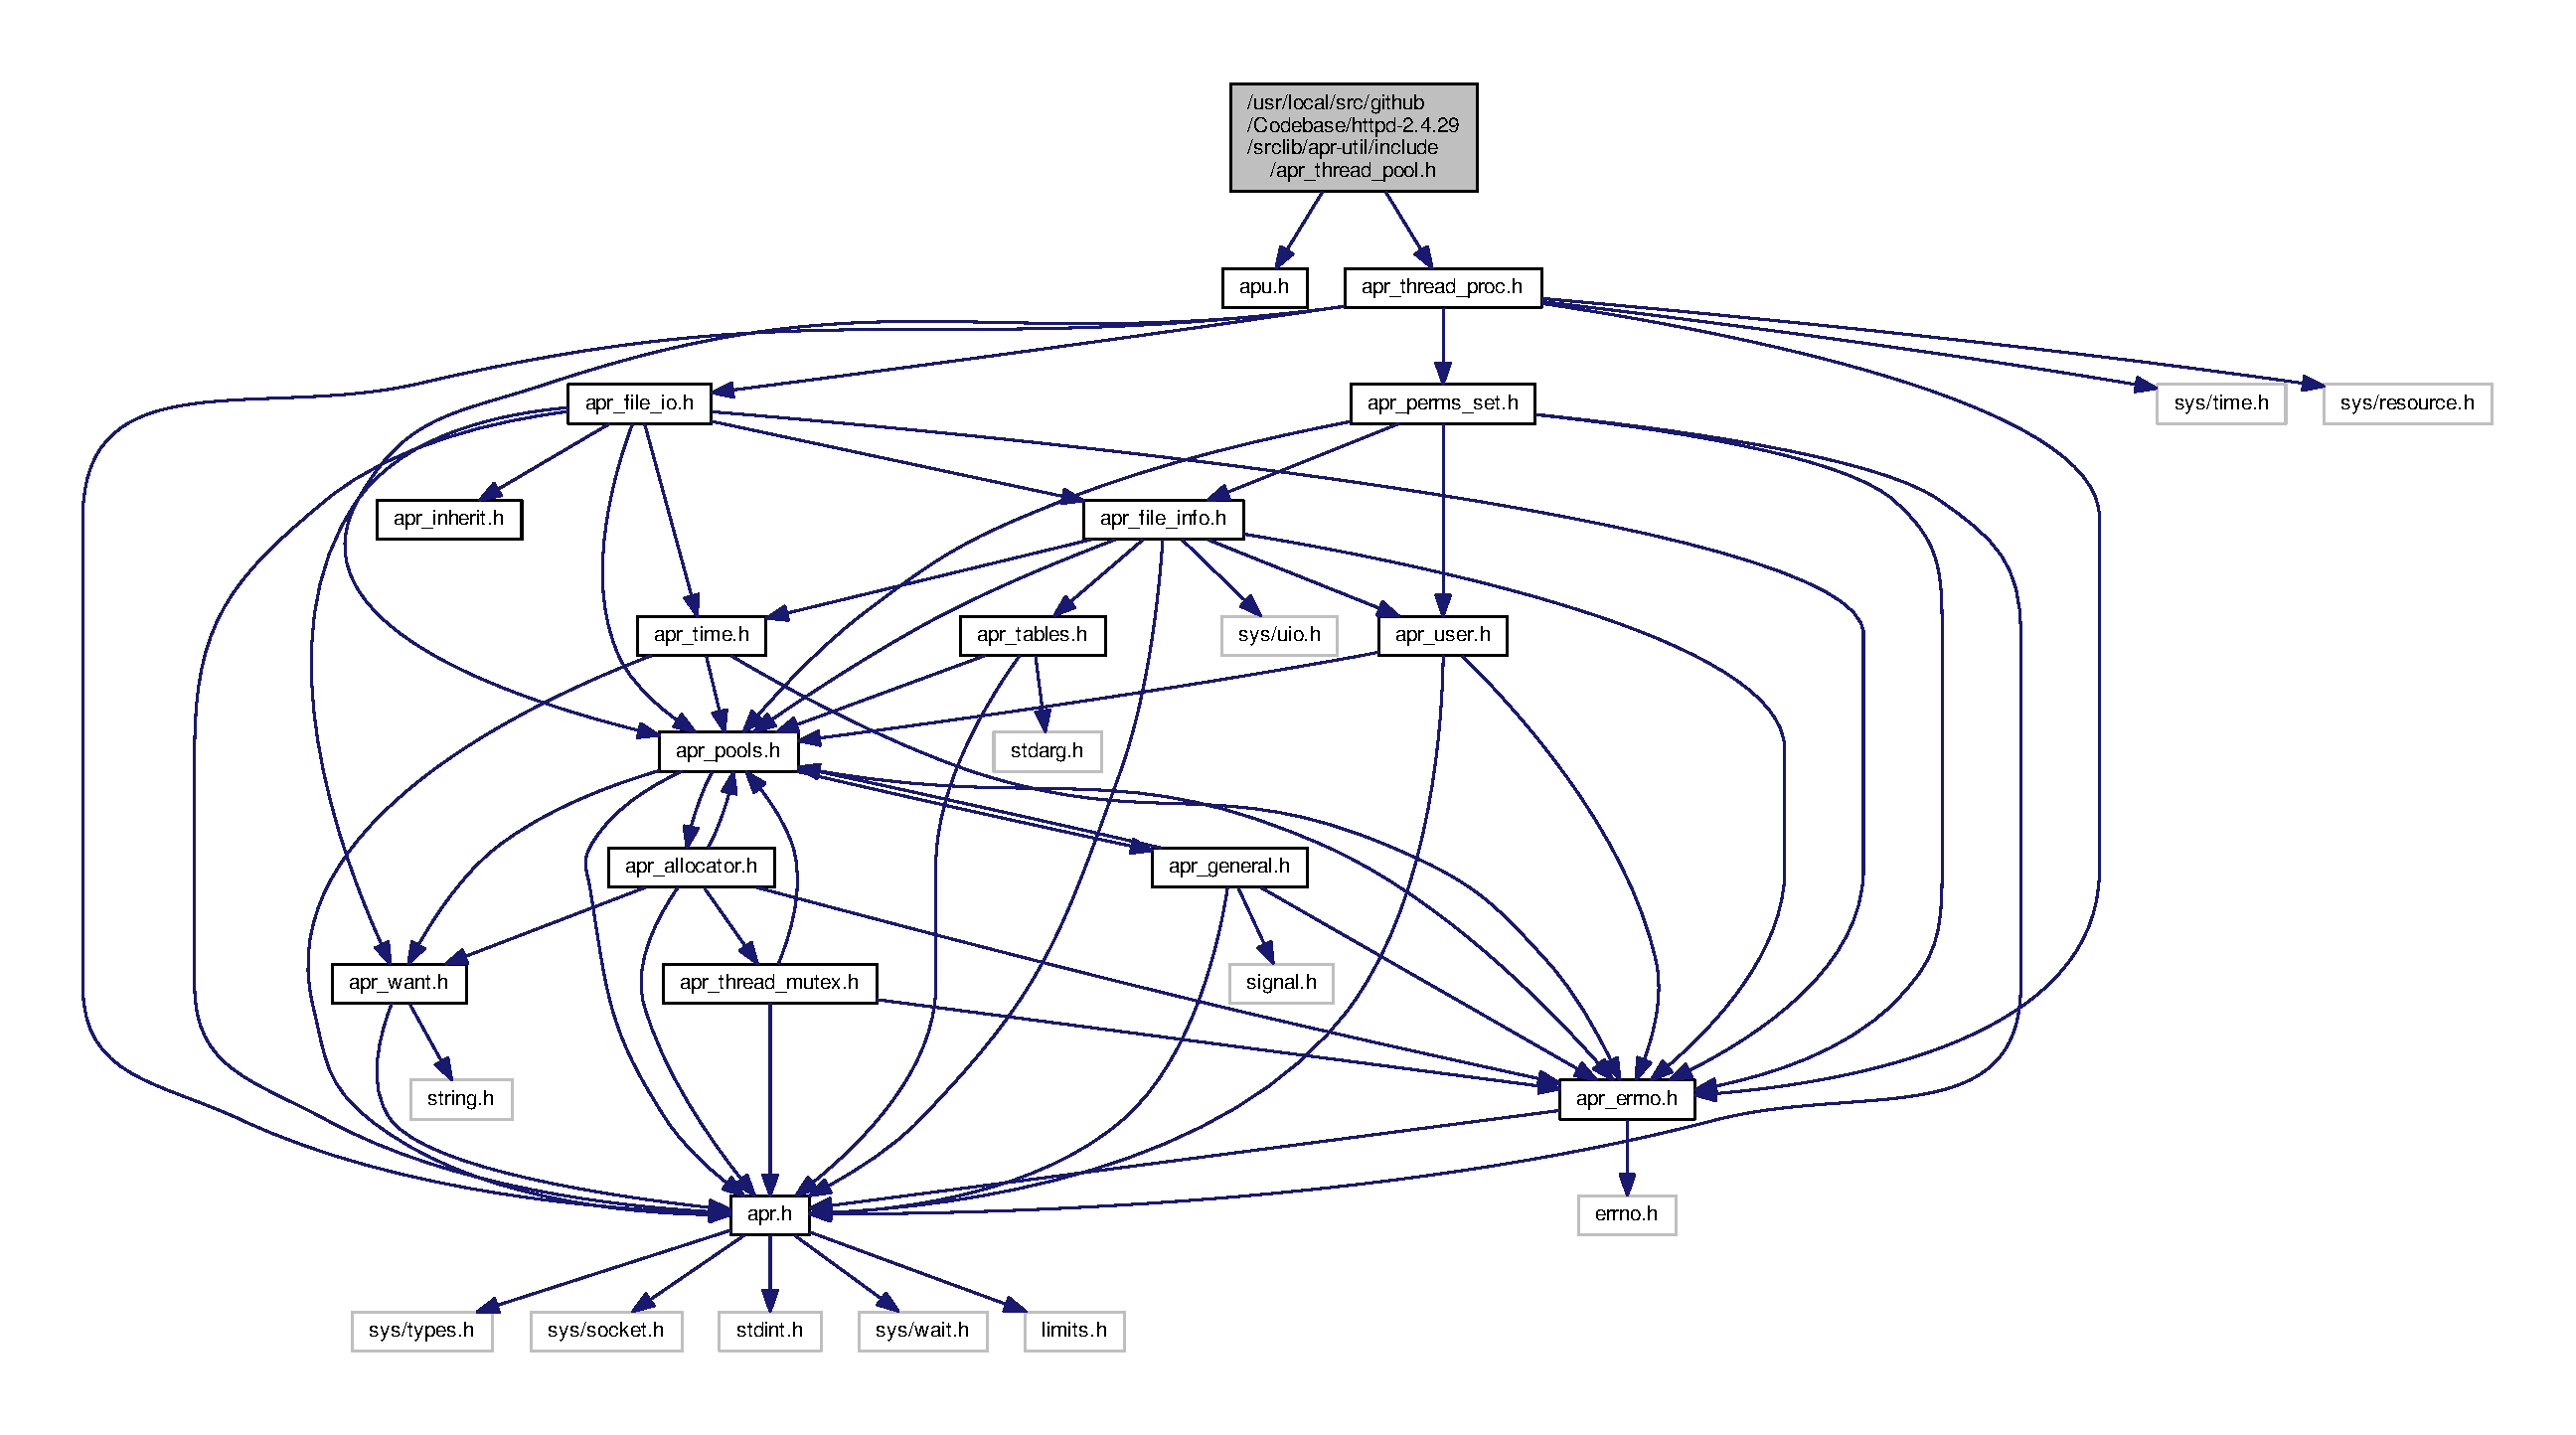
\includegraphics[width=350pt]{apr__thread__pool_8h__incl}
\end{center}
\end{figure}
This graph shows which files directly or indirectly include this file\+:
\nopagebreak
\begin{figure}[H]
\begin{center}
\leavevmode
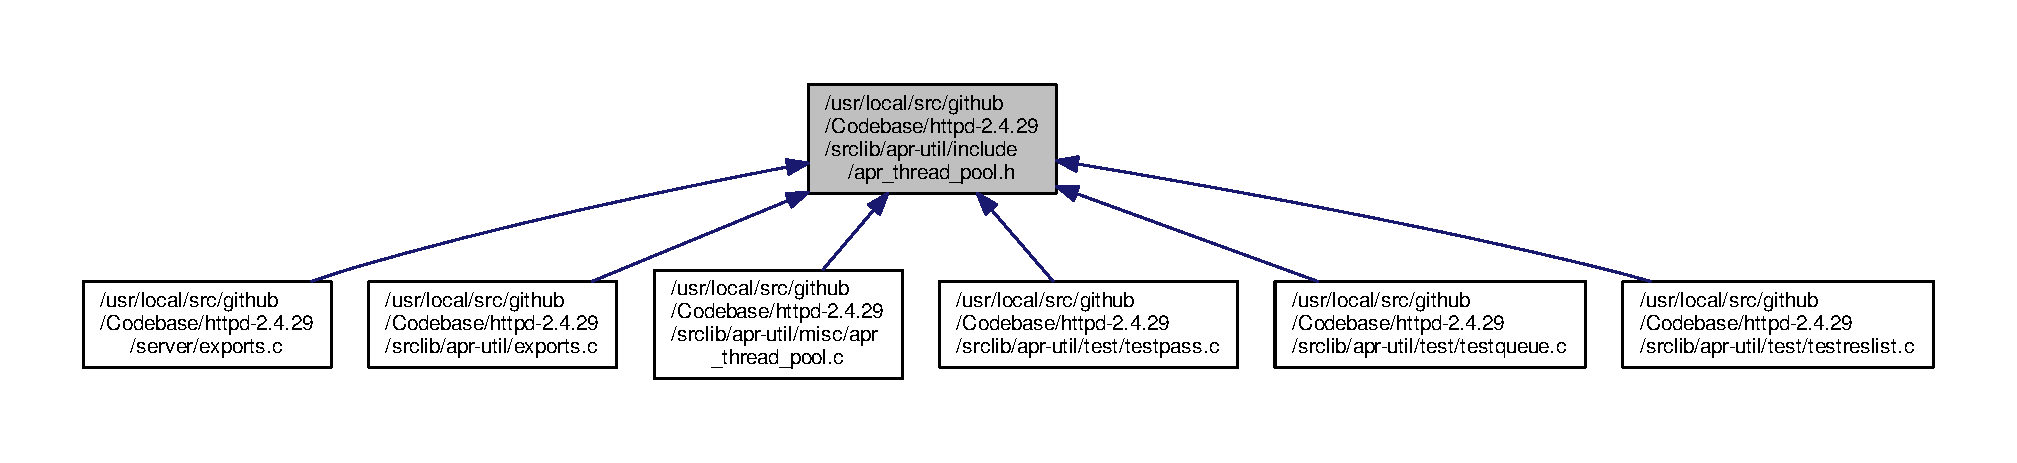
\includegraphics[width=350pt]{apr__thread__pool_8h__dep__incl}
\end{center}
\end{figure}


\subsection{Detailed Description}
A\+PR Thread Pool Library. 

\begin{DoxyRemark}{Remarks}
This library implements a thread pool using \hyperlink{structapr__thread__t}{apr\+\_\+thread\+\_\+t}. A thread pool is a set of threads that can be created in advance or on demand until a maximum number. When a task is scheduled, the thread pool will find an idle thread to handle the task. In case all existing threads are busy and the number of tasks in the queue is higher than the adjustable threshold, the pool will try to create a new thread to serve the task if the maximum number has not been reached. Otherwise, the task will be put into a queue based on priority, which can be valued from 0 to 255, with higher values being served first. If there are tasks with the same priority, the new task might be put at the top or at the bottom -\/ it depends on which function is used to put the task.

There may be the case where the thread pool can use up to the maximum number of threads at peak load, but having those threads idle afterwards. A maximum number of idle threads can be set so that the extra idling threads will be terminated to save system resources. 
\end{DoxyRemark}
